\section{Hyper parameter tuning}

Hyper parameters used in the first model which may be object to optimize are:
\begin{enumerate}
    \item Training data:
    \begin{tasks}(2)
        \task Number of training examples\footnote{Or augmenting the existing training data}
        \task Image size
        \task Batch size
        \task Input color\footnote{It may be useful to set images to grayscale to divide the input size by three}
    \end{tasks}
    \item Model:
    \begin{tasks}(2)
        \task Number of layers
        \task Layer type
        \task Layer size
        \task Loss function
    \end{tasks}
    \item Optimizer:
    \begin{tasks}(2)
        \task Learning rate
        \task Momentum
        \task Decay
        \task Nesterov
    \end{tasks}
    \item Training:
    \begin{tasks}(2)
        \task Steps per epoch
        \task Number of epochs
    \end{tasks}
\end{enumerate}
% TODO the footnotes in this list are not working

Some hyper parameters have to be tested and are not obvious, but others can be improved without any obvious negative side effects so they are discussed first. Then algorithms to test different models with different hyper parameters are explored to improve the model.

\subsection{Data augmentation}
% TODO Add citation to Chollet p.138
% TODO Add dropout layer Chollet p.140
The first thing which can be improved is the size of the dataset we use to train the model.
Since the model shows signs of overfitting and the model sees every image 20 times during training (batches of size 20, 20 steps per epoch and 20 epochs divided by 400 training samples) to increase the training set size is a reasonable approach.
Data augmentation on images changes some properties of the image which are reasonable for the purpose at hand.
In the case of symbol detection the symbol may be rotated or mirrored thus adding training examples without adding much redundancy to the dataset.

Data augmentation is performed by adjusting the \code{create\_generator} function used before:

\begin{lstlisting}
from tensorflow.keras.preprocessing.image import ImageDataGenerator

def create_generator(data_dir, batch_size, datagen):
    full_path = join(processed, data_dir)
    return datagen.flow_from_directory(
        full_path,
        target_size=(32, 32),
        batch_size=batch_size,
        class_mode='binary')

train_datagen = ImageDataGenerator(
        rescale = 1./255,
        rotation_range=360,
        horizontal_flip=True,
        vertical_flip=True)

test_datagen = ImageDataGenerator(rescale = 1./255)

train_generator = create_generator('train', 20, train_datagen)
test_generator = create_generator('test', 10, test_datagen)
\end{lstlisting}

Instead of \code{datagen = ImageDataGenerator(rescale = 1./255)} this object is given as parameter, because the training set adds random deviations to the data loaded. Namely a random rotation and a chance to be horizontally and vertically flipped.
Please note that no deviations are applied to the test data.

Applying these changes gives a loss of 0.61 and a 78.75\% accurarcy on the training data.
Loss and accuracy on the test set are 0.63 and 78\% respectively.

\begin{figure} \label{fig:first_model_data_augmentation_graphs}
    \centering
    \begin{subfigure}[b]{0.4\textwidth}
        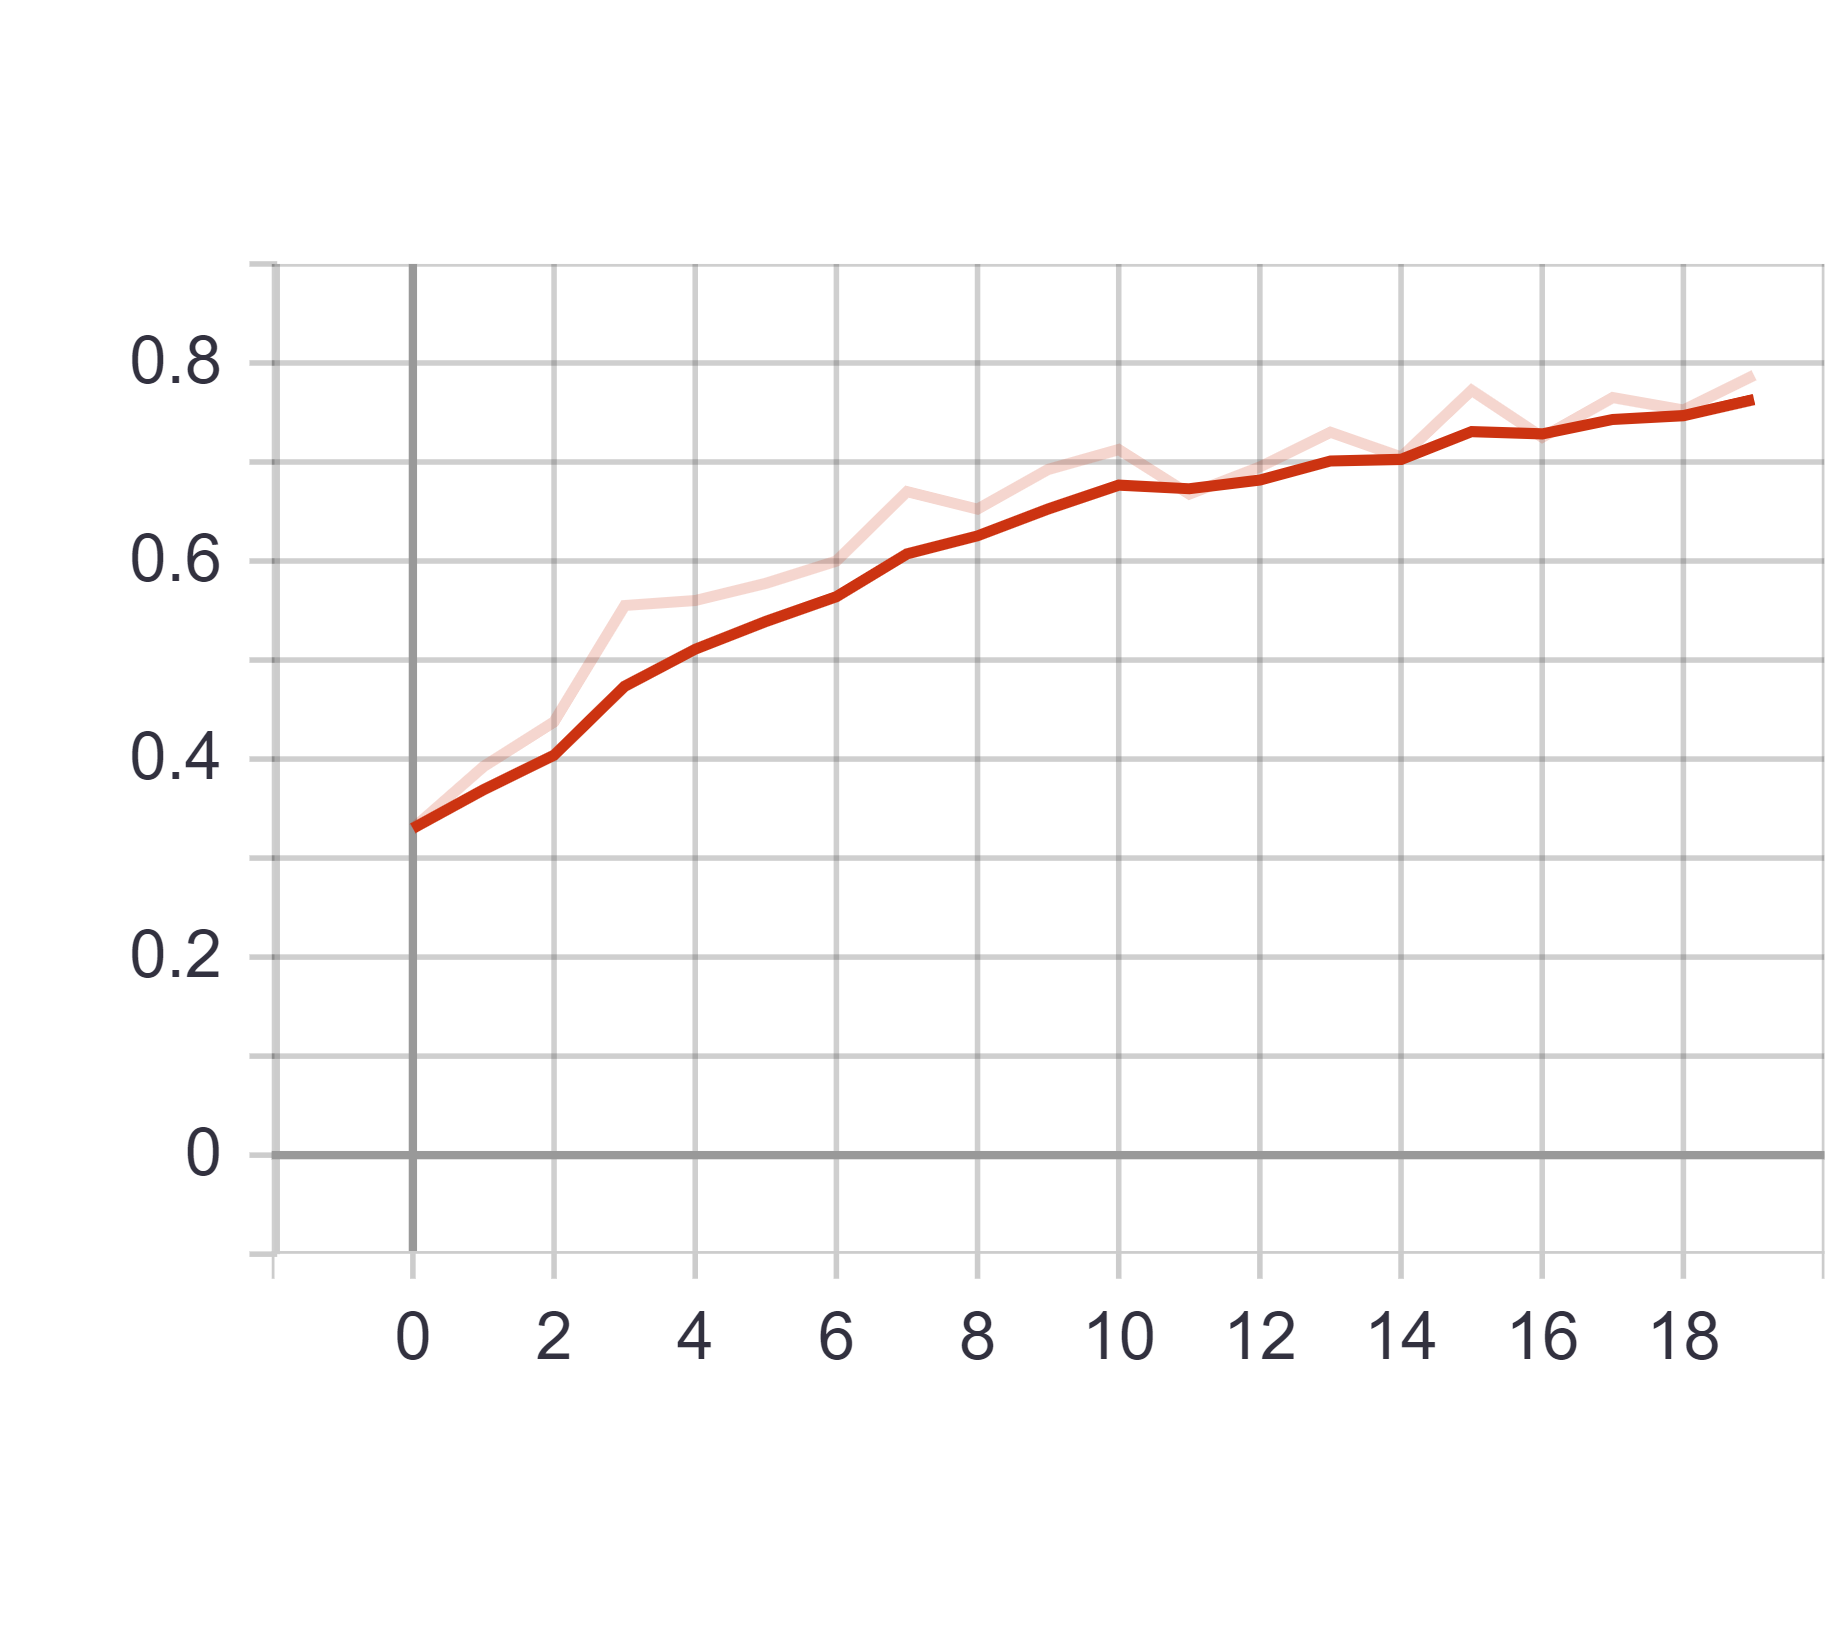
\includegraphics[width=\textwidth]{images/first_model_data_augmentation_acc.png}
        \caption{Accuracy}
        \label{fig:first_model_data_augmentation_acc}
    \end{subfigure}
    \begin{subfigure}[b]{0.4\textwidth}
        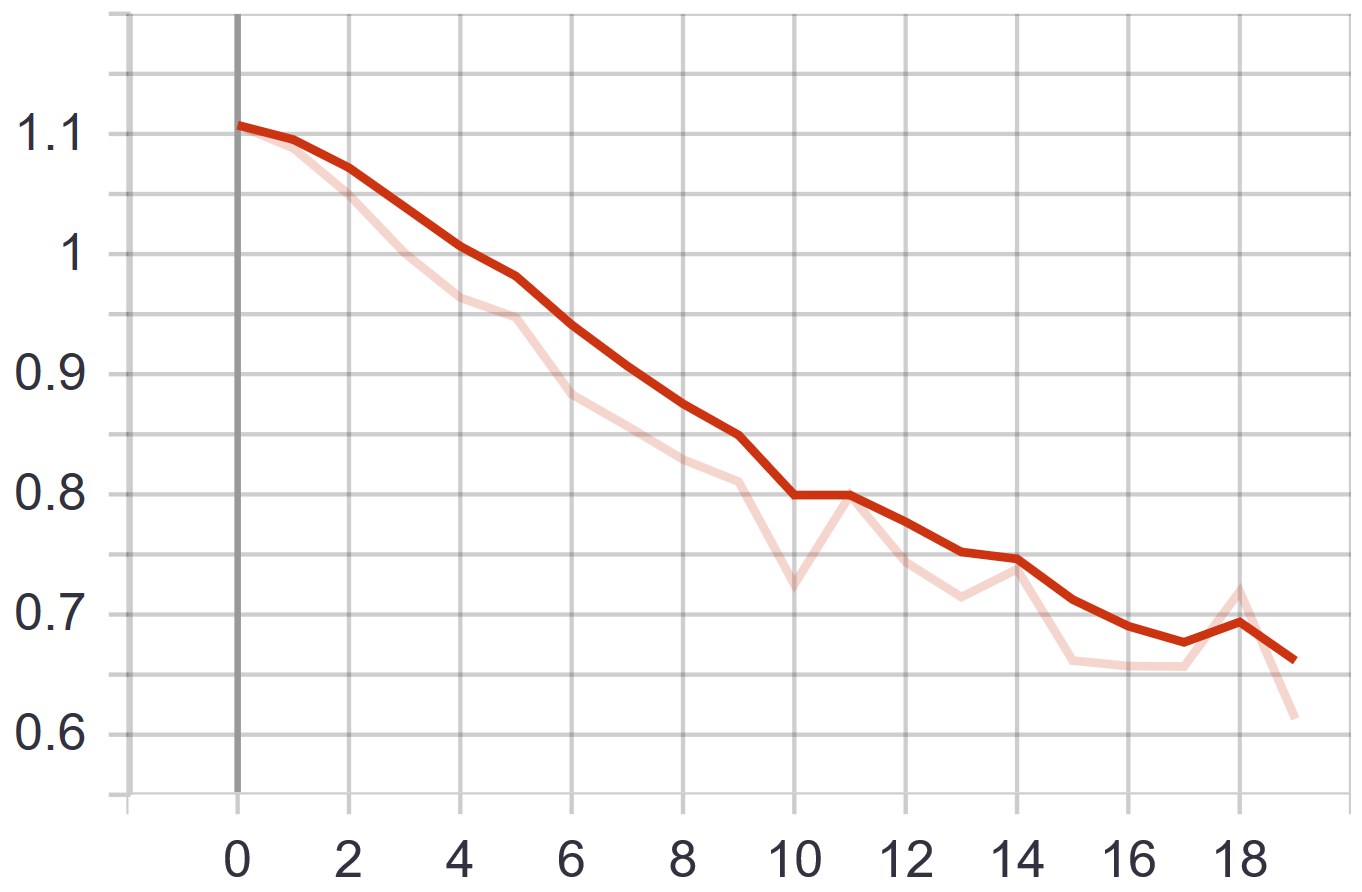
\includegraphics[width=\textwidth]{images/first_model_data_augmentation_loss.png}
        \caption{Loss}
        \label{fig:first_model_data_augmentation_loss}
    \end{subfigure}
    \caption{In comparison to figure~\ref{fig:first_model_graphs} the accuracy and loss are increasing at slower pace. More epochs may improve the results do not seem to be converging after 20 epochs.}
\end{figure}

So it is obvious that accuracy on the training data actually decreased.
This is not surprising, since no data is given twice to the model anymore, so no memorization is happening.
The model accuracy on the training set also seems to be increasing at a lower rate.
More epochs or bigger batches may resolve that problem.

The target to decrease overfitting seems to be resolved this since the difference between training accuracy and test accuracy is negligible small.

\subsection{Grid search}
One way to adjust hyper parameters is to test each with various values alongside all other hyper parameters being fixed.
This procedure ensures that the optimal set of hyper parameters is used, but may take an inacceptable amount of time, since the number of models created is exponentially growing to the number of hyper parameters which are do be adjusted.
If we had two hyper parameters, this would be equivalent to checking every value on a two dimensional grid, hence the name\footnote{If only one hyper parameter is adjusted the procedure is called linear search.}.
